\section{Prototypes}
To get a clear view of how the different pages will look and catch any early potential design problems, we have created prototypes for each of the different pages. 
We will use these to make the implementation of the different pages easier make ensure that we have a consistent design througout the system. 
The prototypes will not serve as an exact vision of how the pages will look but will instead serve as a guideline to how the page should be set up.
In this section we will look at some of the more interesting prototypes where we have had to make some design choices.
\begin{figure}[H]
    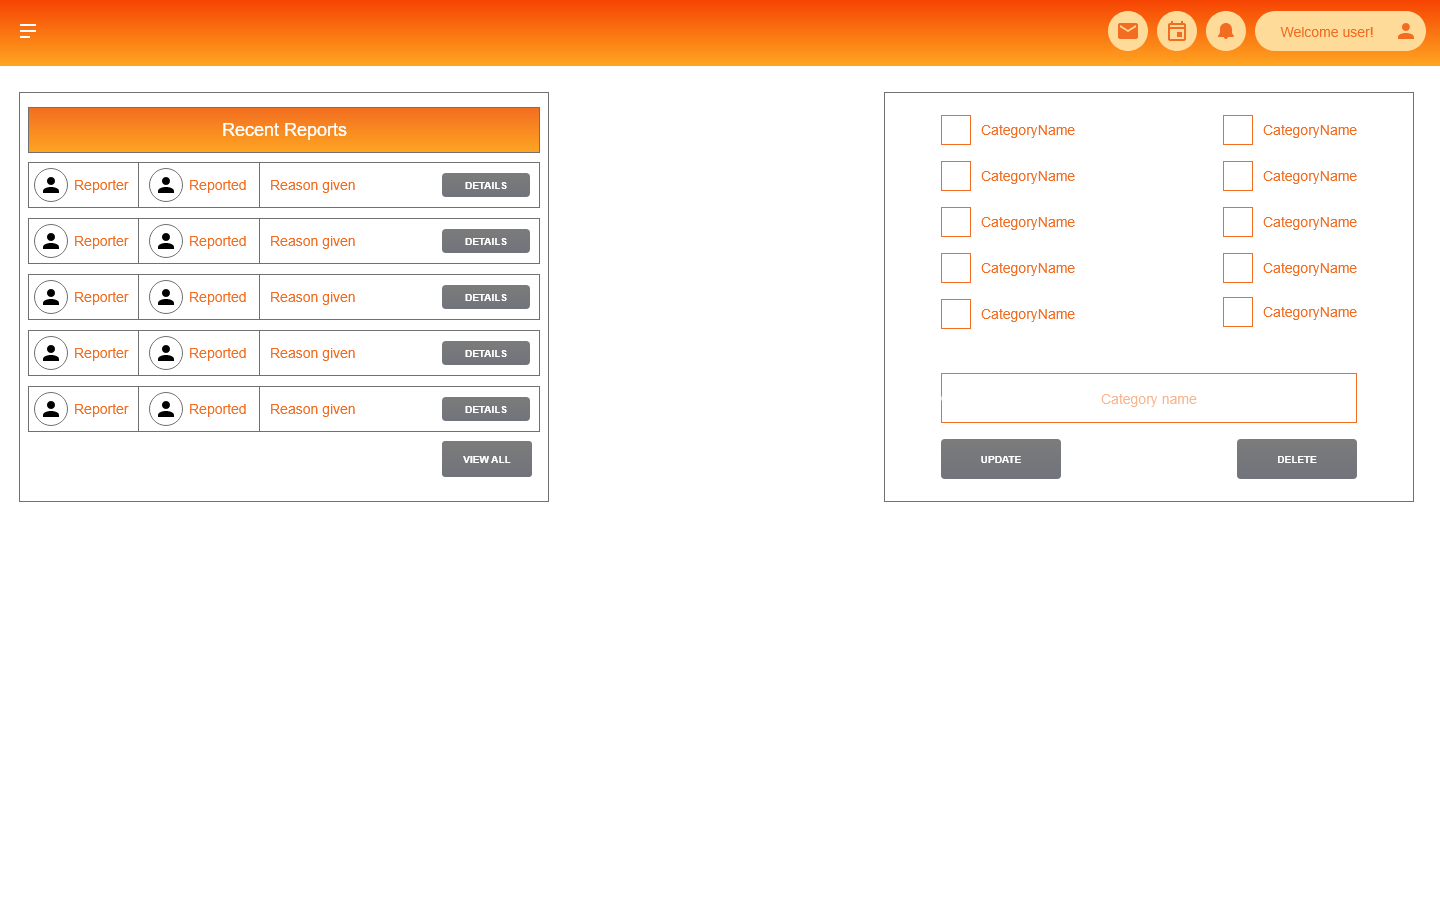
\includegraphics[width=\linewidth]{/prototypes/admin-dashboard.png}
     \caption{Shows the admin dashboard for admins that are logged into the system}
     \label{fig:admin-dashboard}
 \end{figure}
The admin dashboard gives the admin an overview of the recently reported tutors and the different categories. 
The admin needs to see tutor reports since they are the once that will handle them and decide if they should be banned. 
Admins are also in charge of the different teaching categories and therefore they need to have an overview of the current ones and also be able to add new.
We also have a top bar that is used on every page for when the user is logged in. It shows a couple of different icons where the user can go to the inbox, the calendar or the user's own page. It will also show notifications for when different events related to the user happens in the system. On the far left side of the top bar we consider having an icon to go to the landing page but this have not been decided yet
\begin{figure}[H]
   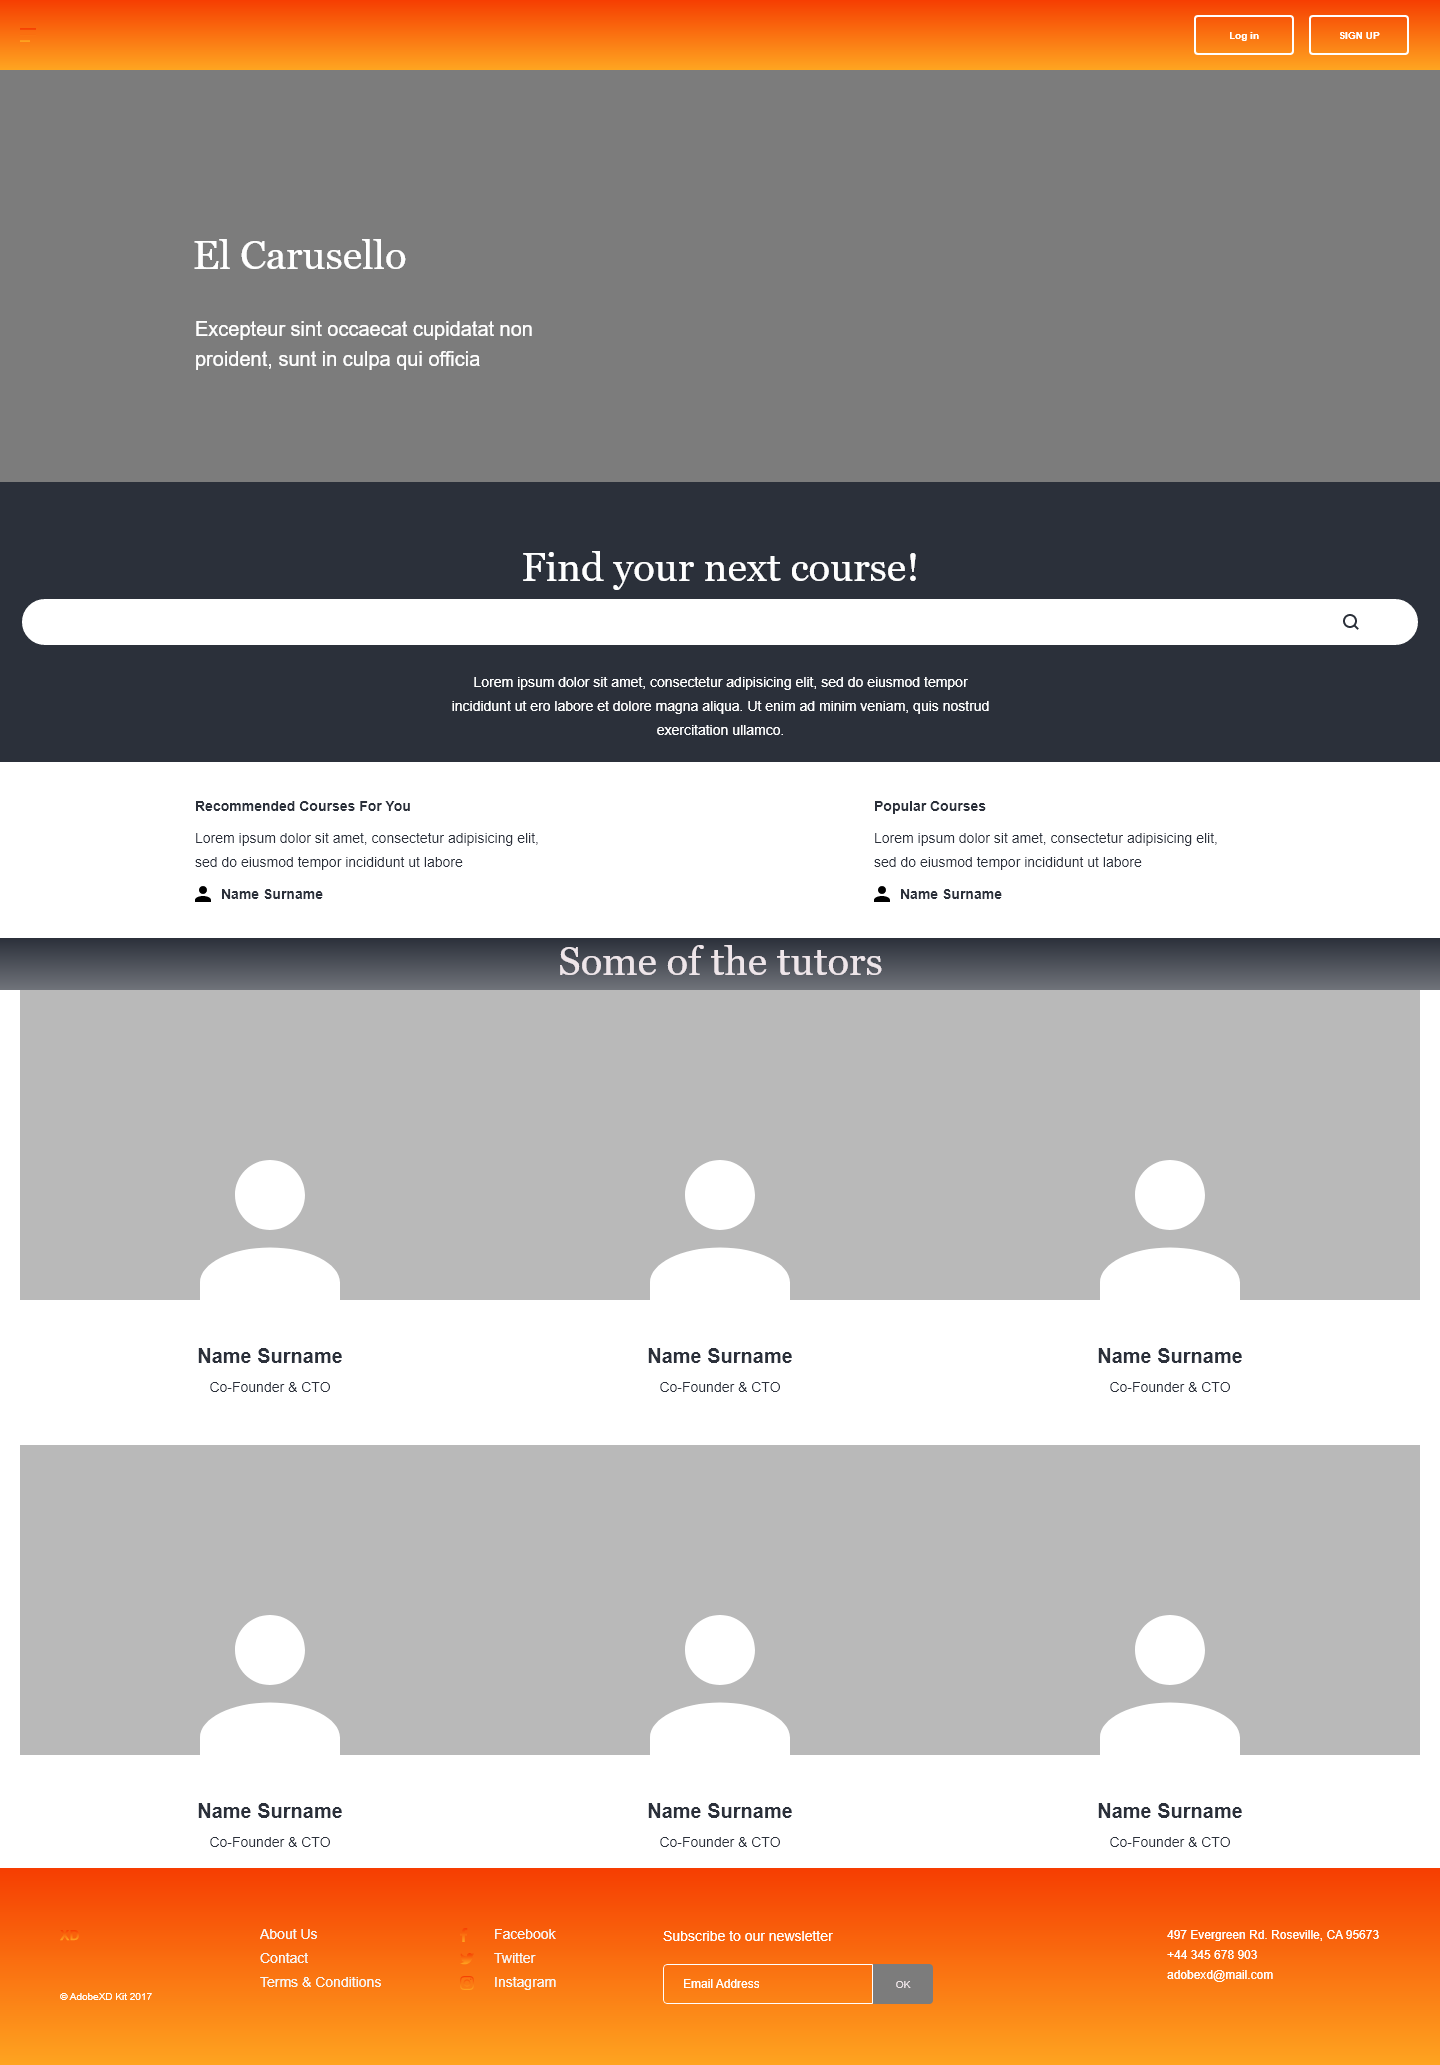
\includegraphics[width=\linewidth, scale=0.5]{/prototypes/landing-page.png}
    \caption{The landing page for the system}
    \label{fig:landing-page}
\end{figure}
The landing page is the first page that the users of the system will see, and thus it is important that this page shows some interesting content. 
This page can be accessed both with and without being logged in. 
We have a top bar that change depending on if the user is logged in or not. 
In the top we will have a carousel that shows some hype images.
Underneath we have a search functionality to find a course or a specific tutor. 
The user should be able to search for both tutors and courses. 
Finally there will be some recommendations for the user which will suggest specific tutors and also show the most popular courses. 

 \begin{figure}[H]
    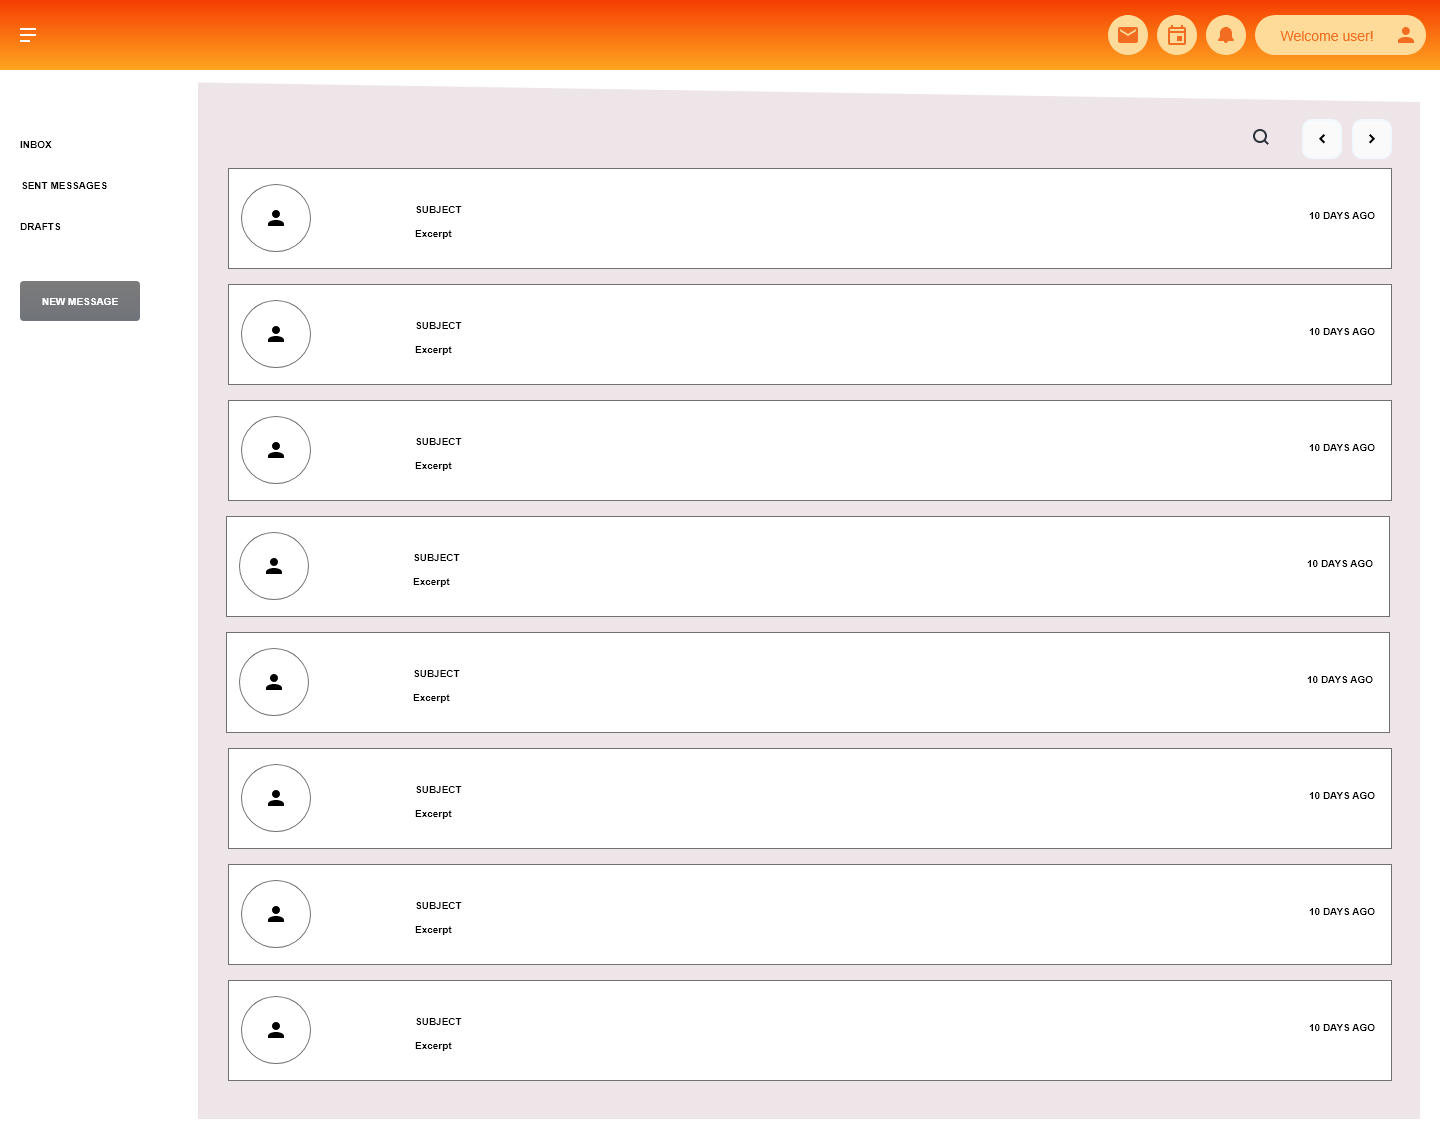
\includegraphics[width=\linewidth]{/prototypes/inbox.png}
     \caption{The inbox for the messaging component in the system}
     \label{fig:inbox}
 \end{figure}
When the user clicks the message icon in the top bar they will be redirected to the inbox page. Here they can view their recent messages. 
We might also include a search functionality to find specific messages. 
The most recently received messages should be shown on the top of the list so they are easy to find. 
When a message is received the topbar should also show a notification for this. 
There should also be something to indicate that a message is unread. 
The user can click a button on the left side of the page to start writing a new message. 


 \begin{figure}[H]
    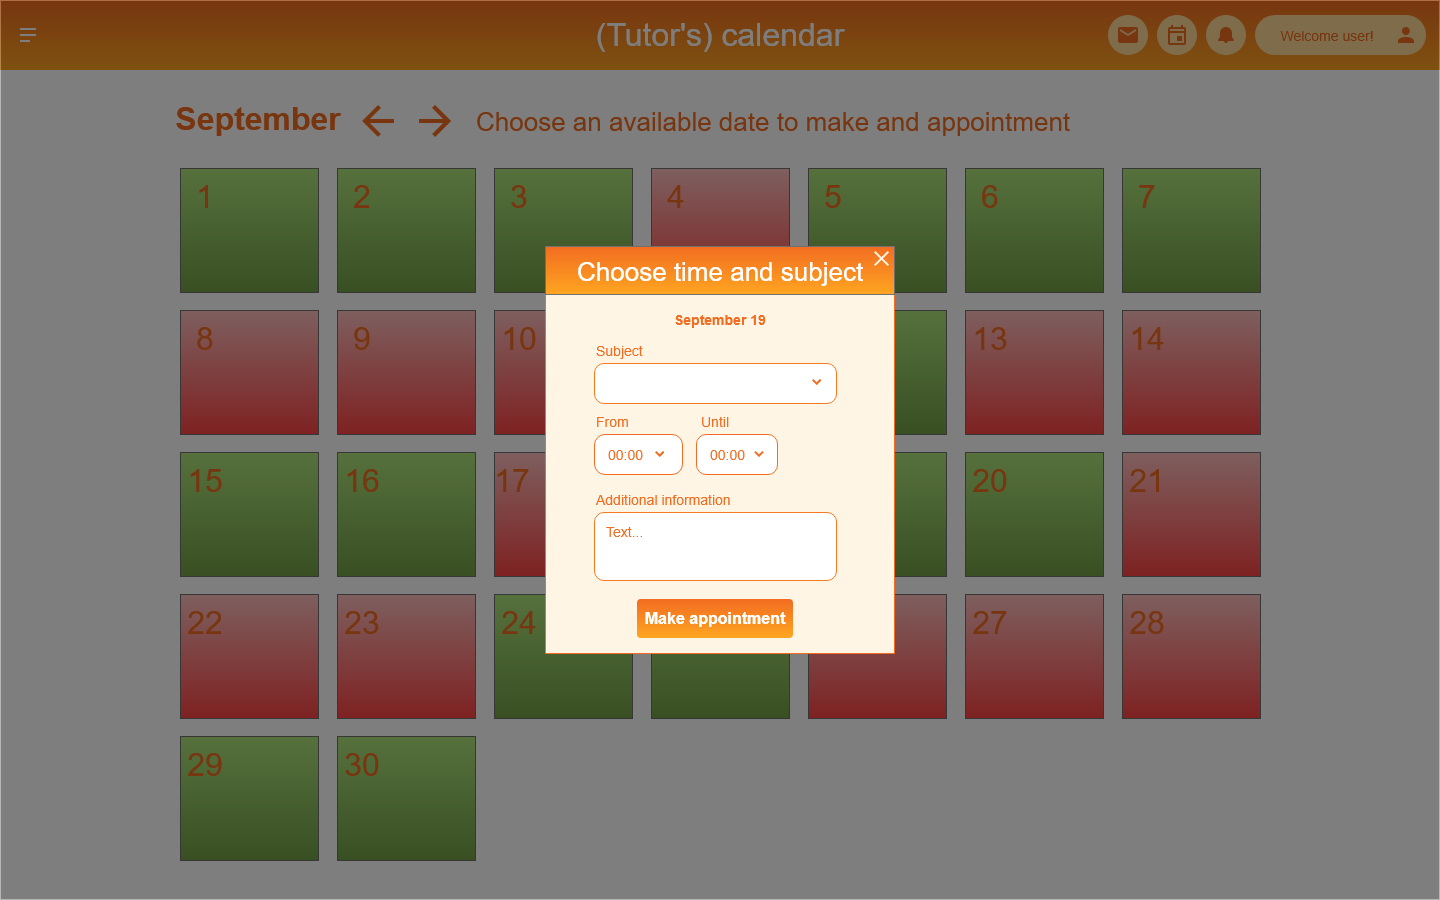
\includegraphics[width=\linewidth]{/prototypes/make-appointment.png}
     \caption{Page that shows a tutor's calendar where the student can request an appointment}
     \label{fig:make-appointment}
 \end{figure}
 This page is the tutor's calendar from a student's point of view. 
 The student is able to browse the tutor's calendar and look for a date where the tutor is available, shown as the color green. 
 The student then clicks the desired date and the popup window will show. 
 Here they can specify the subject they wish to be tought and the timeslot as well as additional information. 
 They can only choose one of tutors available subjects, and the timeslot should comply with the tutor's availability. 
 The tutor also needs to choose what time they are available prior to this.
 When the student makes the appointment they will be sent to a payment page, and a request will be sent to the tutor which they can either accept or deny. 

 \begin{figure}[H]
    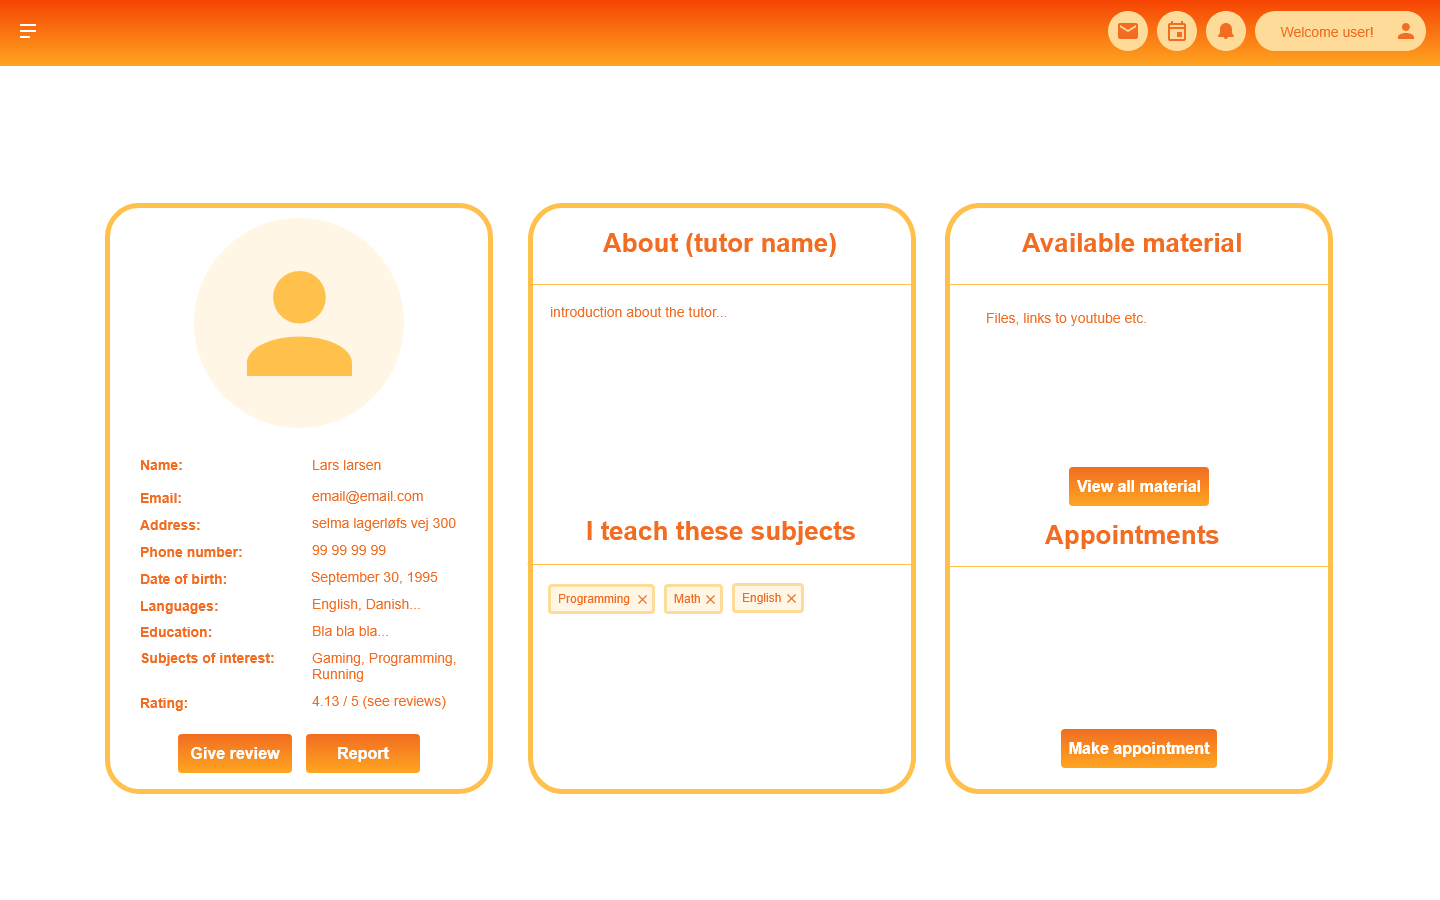
\includegraphics[width=\linewidth]{/prototypes/view-information-on-tutor.png}
     \caption{The page where other users can view information about a specific tutor}
     \label{fig:view-information-on-tutor}
 \end{figure}


 \begin{figure}[H]
    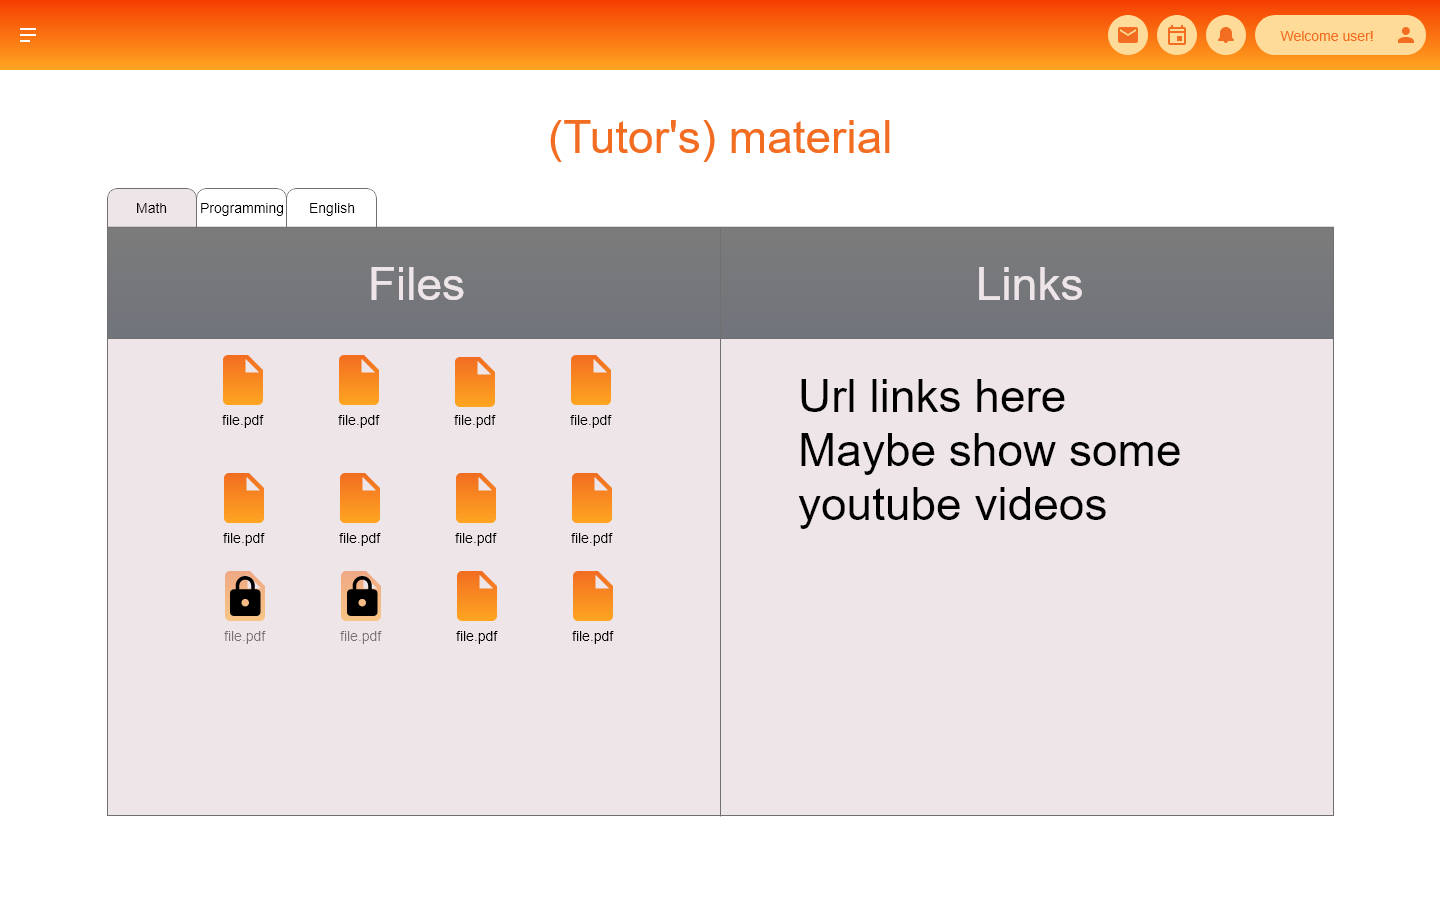
\includegraphics[width=\linewidth]{/prototypes/view-tutor-material.png}
     \caption{The landing page for the system}
     \label{fig:view-tutor-material}
 \end{figure}
